\documentclass[pdftex,a4paper,12pt]{article}
%\usepackage{pscyr}
\usepackage[T2A]{fontenc}
\usepackage[russian]{babel}
\usepackage[utf8]{inputenc}
\usepackage{lmodern}
\usepackage{graphicx}

\title{Численное моделирование фильтра циклон}
\author{Дмитрий Богданов}
\date{}
\begin{document}
\renewcommand\normalsize{\fontsize{12pt}{14pt}\selectfont}
\begin{titlepage}
	\begin{center}
		\small{МИНИСТЕРСТВО ОБРАЗОВАНИЯ И НАУКИ \\ РОССИЙСКОЙ ФЕДЕРАЦИИ \\
Санкт-Петербургский государственный политехнический университет \\
Физико-механический факультет \\
Кафедра гидроаэродинамики}\\
		\vspace{0.18\textheight}
	\end{center}
	\begin{center}
		\vspace{0.1\textheight}
		\large{Численное исследование течения в фильтре-циклоне}\\
		\vspace{0.01\textheight}
		\normalsize
		\textsc{Автореферат диссертации на соискание ученой степени магистра по направлению 010600 – Прикладные математика и физика}
		\vspace{0.25\textheight}
	\end{center}
	\begin{minipage}{0.48\textwidth}
		\begin{flushleft}
			Выполнил студент гр. 6054/11\\
			Руководитель, к.ф.-м.н., с.н.с.\\
		\end{flushleft}
	\end{minipage}
	\begin{minipage}{0.5\textwidth}
		\begin{flushright}
			Богданов Д.А. \\
			Поняев С.А. \\
		\end{flushright}
	\end{minipage}
	\vspace{0.1\textheight}
	\begin{center}
		Санкт-Петербург \\
		\the\year
	\end{center}
\end{titlepage}
\newpage
\renewcommand\normalsize{\fontsize{14pt}{24pt}\selectfont}
\tableofcontents
\newpage
\section{Введение}
\subsection{Актуальность проблемы}
	\hspace{2em} 	Задача очищения атмосферного воздуха от загрязняющих выбросов промышленных предприятий достаточно актуальна. Выбросы от стационарных источников вредных веществ в атмосферу городов и населенных пунктов, расположенных на территории северо-западного федерального округа,  по данным Росстата за 2007 год,  составили 2319000 тонн, в том числе твёрдых -- 289400 тонн.
	\begin{figure}[ht]
		\vspace{-1.4em}
		\begin{minipage}[b]{0.48\linewidth}
		По данным European Environment Agency выброс $SO_2$ в европе (за исключением России) за 2010 год составил 8297000 тонн.
			Динамика изменения объёма выбросов твёрдых вредных веществ в атмосферу \textit{(рис. \ref{figure:atmosphereDynamic})} имеет тенденцию к росту, что говорит о том, что решение проблемы инженерной защиты воздуха от вредных веществ останется актуальной и в ближайшем будущем. 
		\end{minipage}
		\hspace{0.04\linewidth}
		\begin{minipage}[b]{0.48\linewidth}
			\centering
			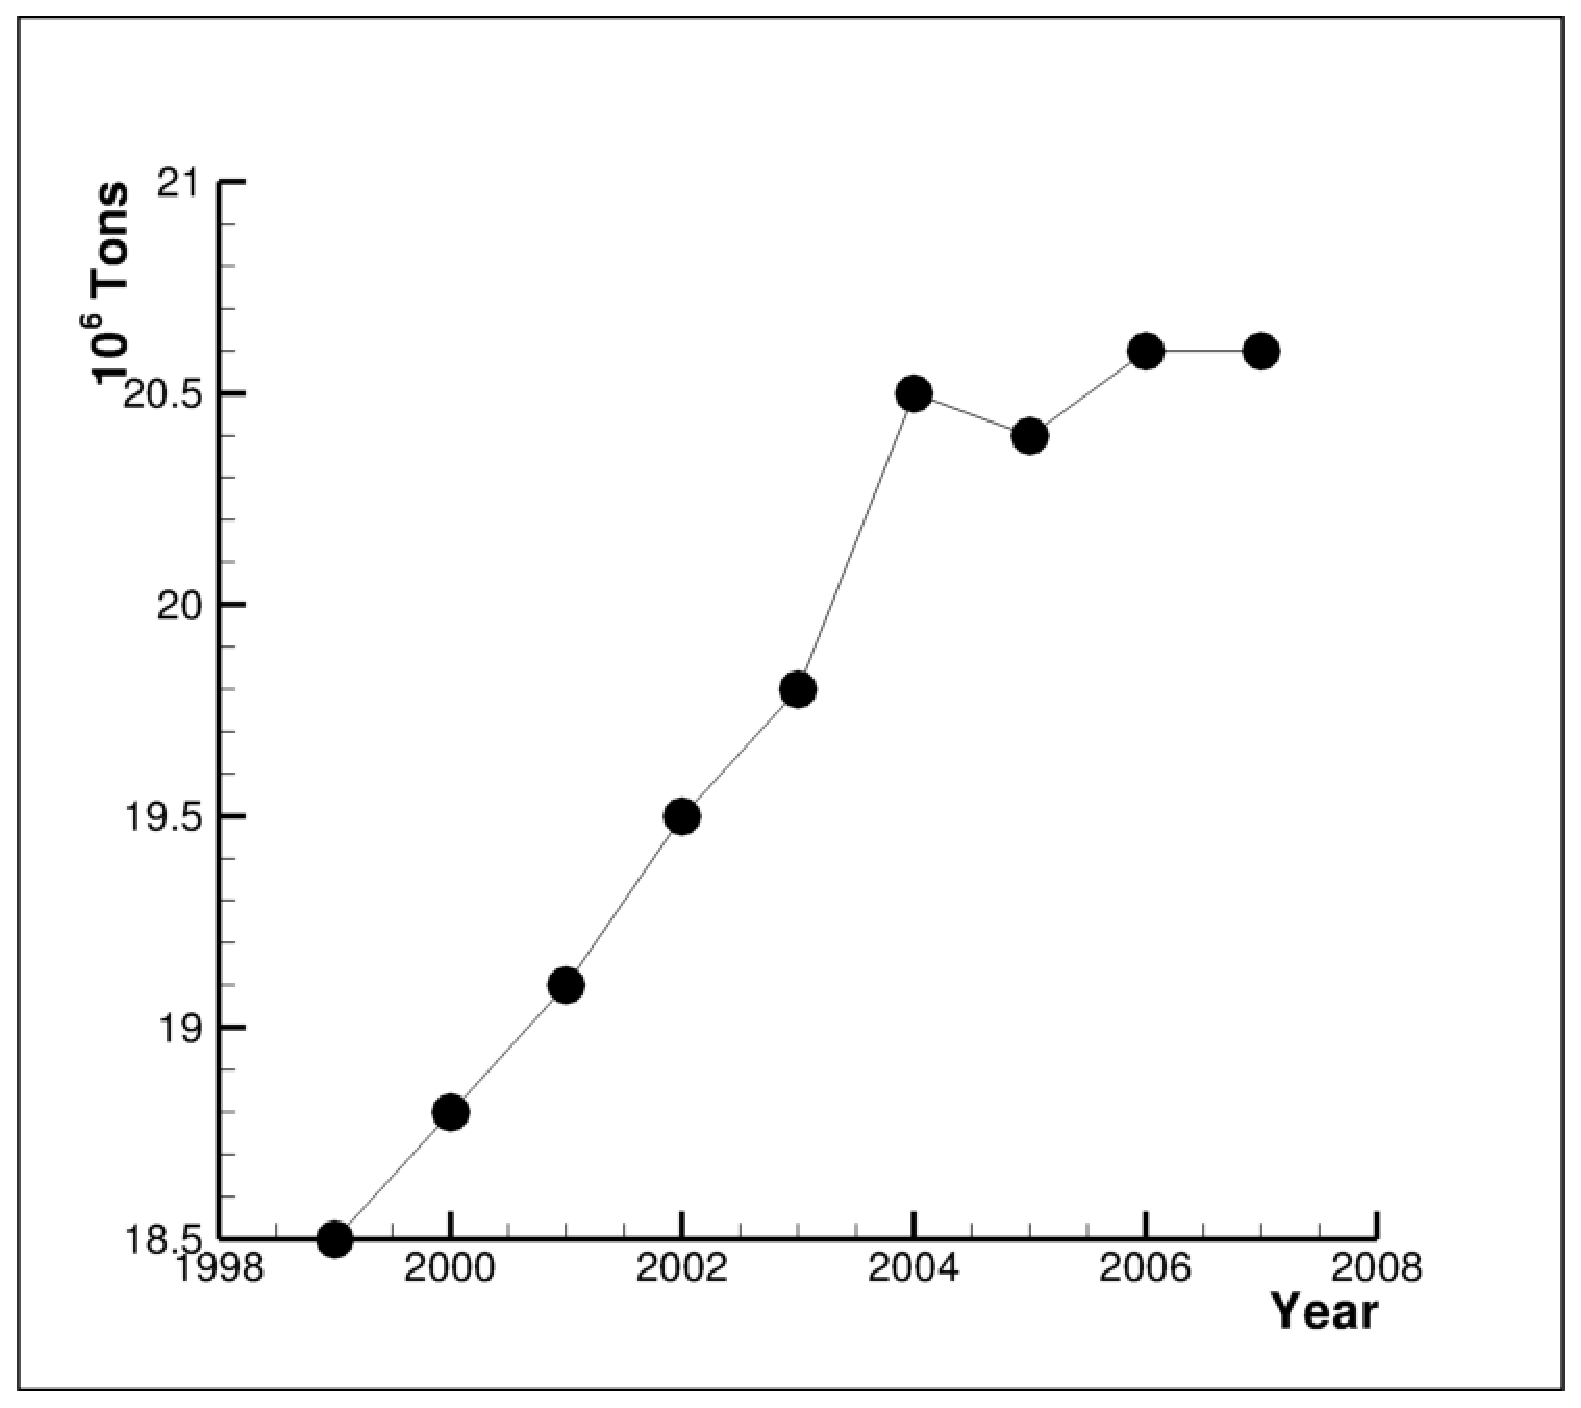
\includegraphics[scale=0.2]{atmosphereDynamic}
			\caption{Динамика выбросов твёрдых вредных веществ в атмосферу}
			\label{figure:atmosphereDynamic}
		\end{minipage}
	\end{figure}
	
	Для очищения воздуха от твёрдых примесей широкое распространение получили фильтры типа циклон. 
	\subsection{Цели работы}
%Введение
\end{document}
